\chapter{提案システム}

\section{概要}
本章では,本研究で提案するシステムについて説明する.
本研究では,識別精度を犠牲にすることなくアノテーションコストを抑えるために能動学習を病理画像解析に取り入れるシステムを構築する.

ここで,本システムの要求機能の詳細を述べる.
\begin{itemize}
    \item[1.] 実用に足る識別精度を達成する予測モデルを獲得できること
    \item[2.] アノテーションコストが出来る限り低いこと
    \item[3.] 現実的な計算コストでクエリを選択可能なアルゴリズムであること
    \item[4.] WSIに含まれる大量に存在するラベルなしデータを扱えること
\end{itemize}

病理医にも匹敵する精度を達成するため,本研究では識別器にConvolutional Neural Network(CNN)を採用する.
また,少ないラベル数でも学習を収束させるためにImageNetで学習済みのモデルの重みをもとにfine-tuningによって学習を行う.
\ref{sec:path_images}節で述べたように,一般画像認識のために学習されたモデルでも,医療画像解析への転移学習は幅広いタスクに対して有効であると知られているため,妥当だと考えられる.

前章で述べたように,多くの能動学習アルゴリズムはCNNのように膨大なパラメータ数を持つアルゴリズムに対して適用する場合計算コストが爆発する問題がある.
さらに,前章で述べたように深層学習と能動学習を組み合わせた手法の多くが採用しているUncertainty Samplingは,不確かさを陽にモデル化しないCNNに対しては相性が良くないと考えられる.
そこで本研究では,深層能動学習の新たな手法として,Query-By-Dropout-Predictionsを提案する.
不確かさを定義しない多層ニューラルネットワークのパラメータを更新するサンプルを効率的に見つけるために,
多層ニューラルネットワークの学習において正則化の目的で使用されるDropoutを利用して擬似的にQuery-By-Committeeを再現する.
さらに,医療画像解析において重要であると考えられる様々な変形への不変性の担保を考慮し,
各Committeeのprediction時にもランダムなData Augmentationを利用することで,
識別に有効なサンプルのみではなく不変性を確保するために有効であるサンプルをクエリとして選択する手法も提案する.

また病理画像は,WSI内に多くの類似画像が存在するため,バッチ内能動学習を採用した場合にクエリ内に類似画像が多数含まれることで,無駄なアノテーションが生じてしまう可能性が高い.
そこで,クラスタリングを事前に行うことでクエリ内の情報重複問題を緩和することを考える.
その際に用いる特徴量について,病理画像パッチはテクスチャとして扱われることが多いという特徴を考慮し,妥当だと考えられるものを列挙した上で実験から選定する.

さらに,病理画像解析に能動学習を適用するためにはWSIに含まれる大量に存在するラベルなしデータを扱う必要がある.
そこでWSIを多数含む病理画像データセットに含まれる大量の画像パッチを最大限に有効活用するための実用的な方法を提案する.

以下の節では,それぞれについて詳細を説明する.

\begin{figure}[tbp]
    \label{fig:overview}
     \begin{center}
      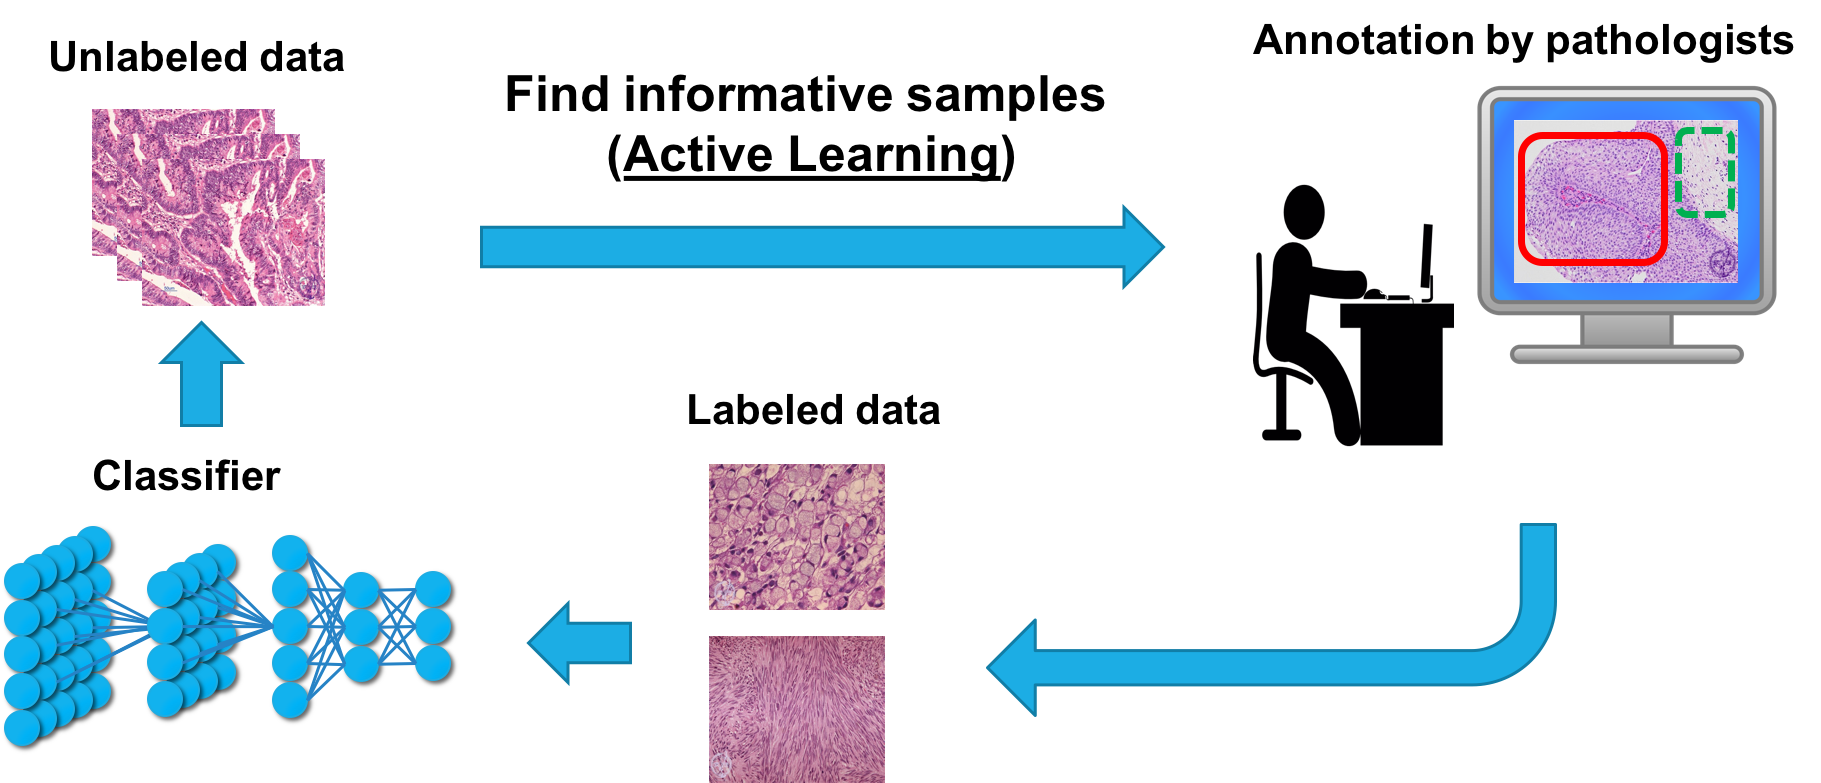
\includegraphics[width=120mm]{figures/overview.png}
     \end{center}
    \caption{本研究で提案するシステムの概念図}
\end{figure}

\section{\textbf{Query by Dropout Predictions}}
\subsection{手法の詳細}
多層ニューラルネットワークによって識別問題を解く際には,最終出力が各ラベルに対応する確率分布となるように設計して学習を行う.
多層ニューラルネットワークを能動学習に利用してUncertainty Samplingによってクエリ選択を行う場合は,
この確率分布のエントロピーの大きさなどを利用して不確かさを定量評価する.
しかし,前章で述べたように,ニューラルネットワーク自体のパラメータに対する不確かさをモデリングしているわけではない.
また,このように不確かさを陽にモデル化しない識別器を利用した能動学習では,
バージョン空間を縮小させるサンプルを選択するQuery By Committee(QBC)\cite{seung1992query}がしばしば用いられる.
このバージョン空間を全て保持するのは多くの識別器において不可能であるため,
現在のラベル付きデータ集合を使用して学習した複数のモデル(Committee)によって近似的に表現する事が多い.
Committeeがバージョン空間を近似するには,以下の条件を満たす必要がある.
\begin{itemize}
\item 現在のラベル付きデータ集合に対してはConsistentであること
\item 未知データに対する予測に分散を持つこと
\end{itemize}
しかし,QBCをCNNに適用することを考えた場合,CNNのように計算コストの重いモデルを複数同時に保持し学習するのは,メモリ,
計算コストの観点から現実的ではない.また,膨大なパラメータ数を持つ多層ニューラルネットワークの最適解の探索空間は非常に広く,
有限個のCommitteeメンバによってバージョン空間を近似するのは難しい.
% 異なる初期値から学習されたメンバの準最適解は大きく異なる可能性が高い.
% 有限個のメンバの予測の不一致度が大きいサンプルが,すべてのメンバの準最適解に向かうために必要であるかは自明ではない.

ここで,多くの深層学習のアーキテクチャにおいて,正則化のために利用されるDropoutによって,
本体のネットワークからサンプリングされた部分ネットワークの性質に着目する.
Dropoutを利用し十分に学習されたネットワークの部分ネットワークは,現在のラベル付きデータに対してはほぼConsistentであると考えられる.
% また,committeeメンバは大部分のパラメータを共有しているため,近傍のバージョン空間を小さくすることができる.
% 異なる初期値から学習されたcommitteeの場合と比較すると一致している可能性が高いと考えられる.

そこで,本研究ではDropoutによってサンプリングされた部分ネットワークの予測の不一致度を利用して
近似的にQuery-By-Committeeを行う手法 Query-By-Dropout-Predictionsを提案する(図\ref{fig:query_by_dropout}).
つまり,本体のネットワーク$\mathcal{M}$から生成された部分ネットワーク$\mathcal{C} = \{\mathcal{M}_{p_1}, \mathcal{M}_{p_2}, \dots, \mathcal{M}_{p_c} \}$を用いて
以下のAverage Kullback Leibler Divergenceを計算する.
\begin{eqnarray}
    score(x) =  -  \frac{1}{C} \sum_{c=i}^C KL \, (P_{\theta^{(c)}} || P_C)
\end{eqnarray}

アルゴリズムの詳細をAlgorithm.\ref{algo:qbdp}に示す.
これらの部分ネットワークがCommitteeのメンバとして利用されるための条件としてあげた2つの性質について実験で検証し,
Uncertainty Samplingのみを利用する方法と比較する.

\begin{figure}[tbp]
     \begin{center}
      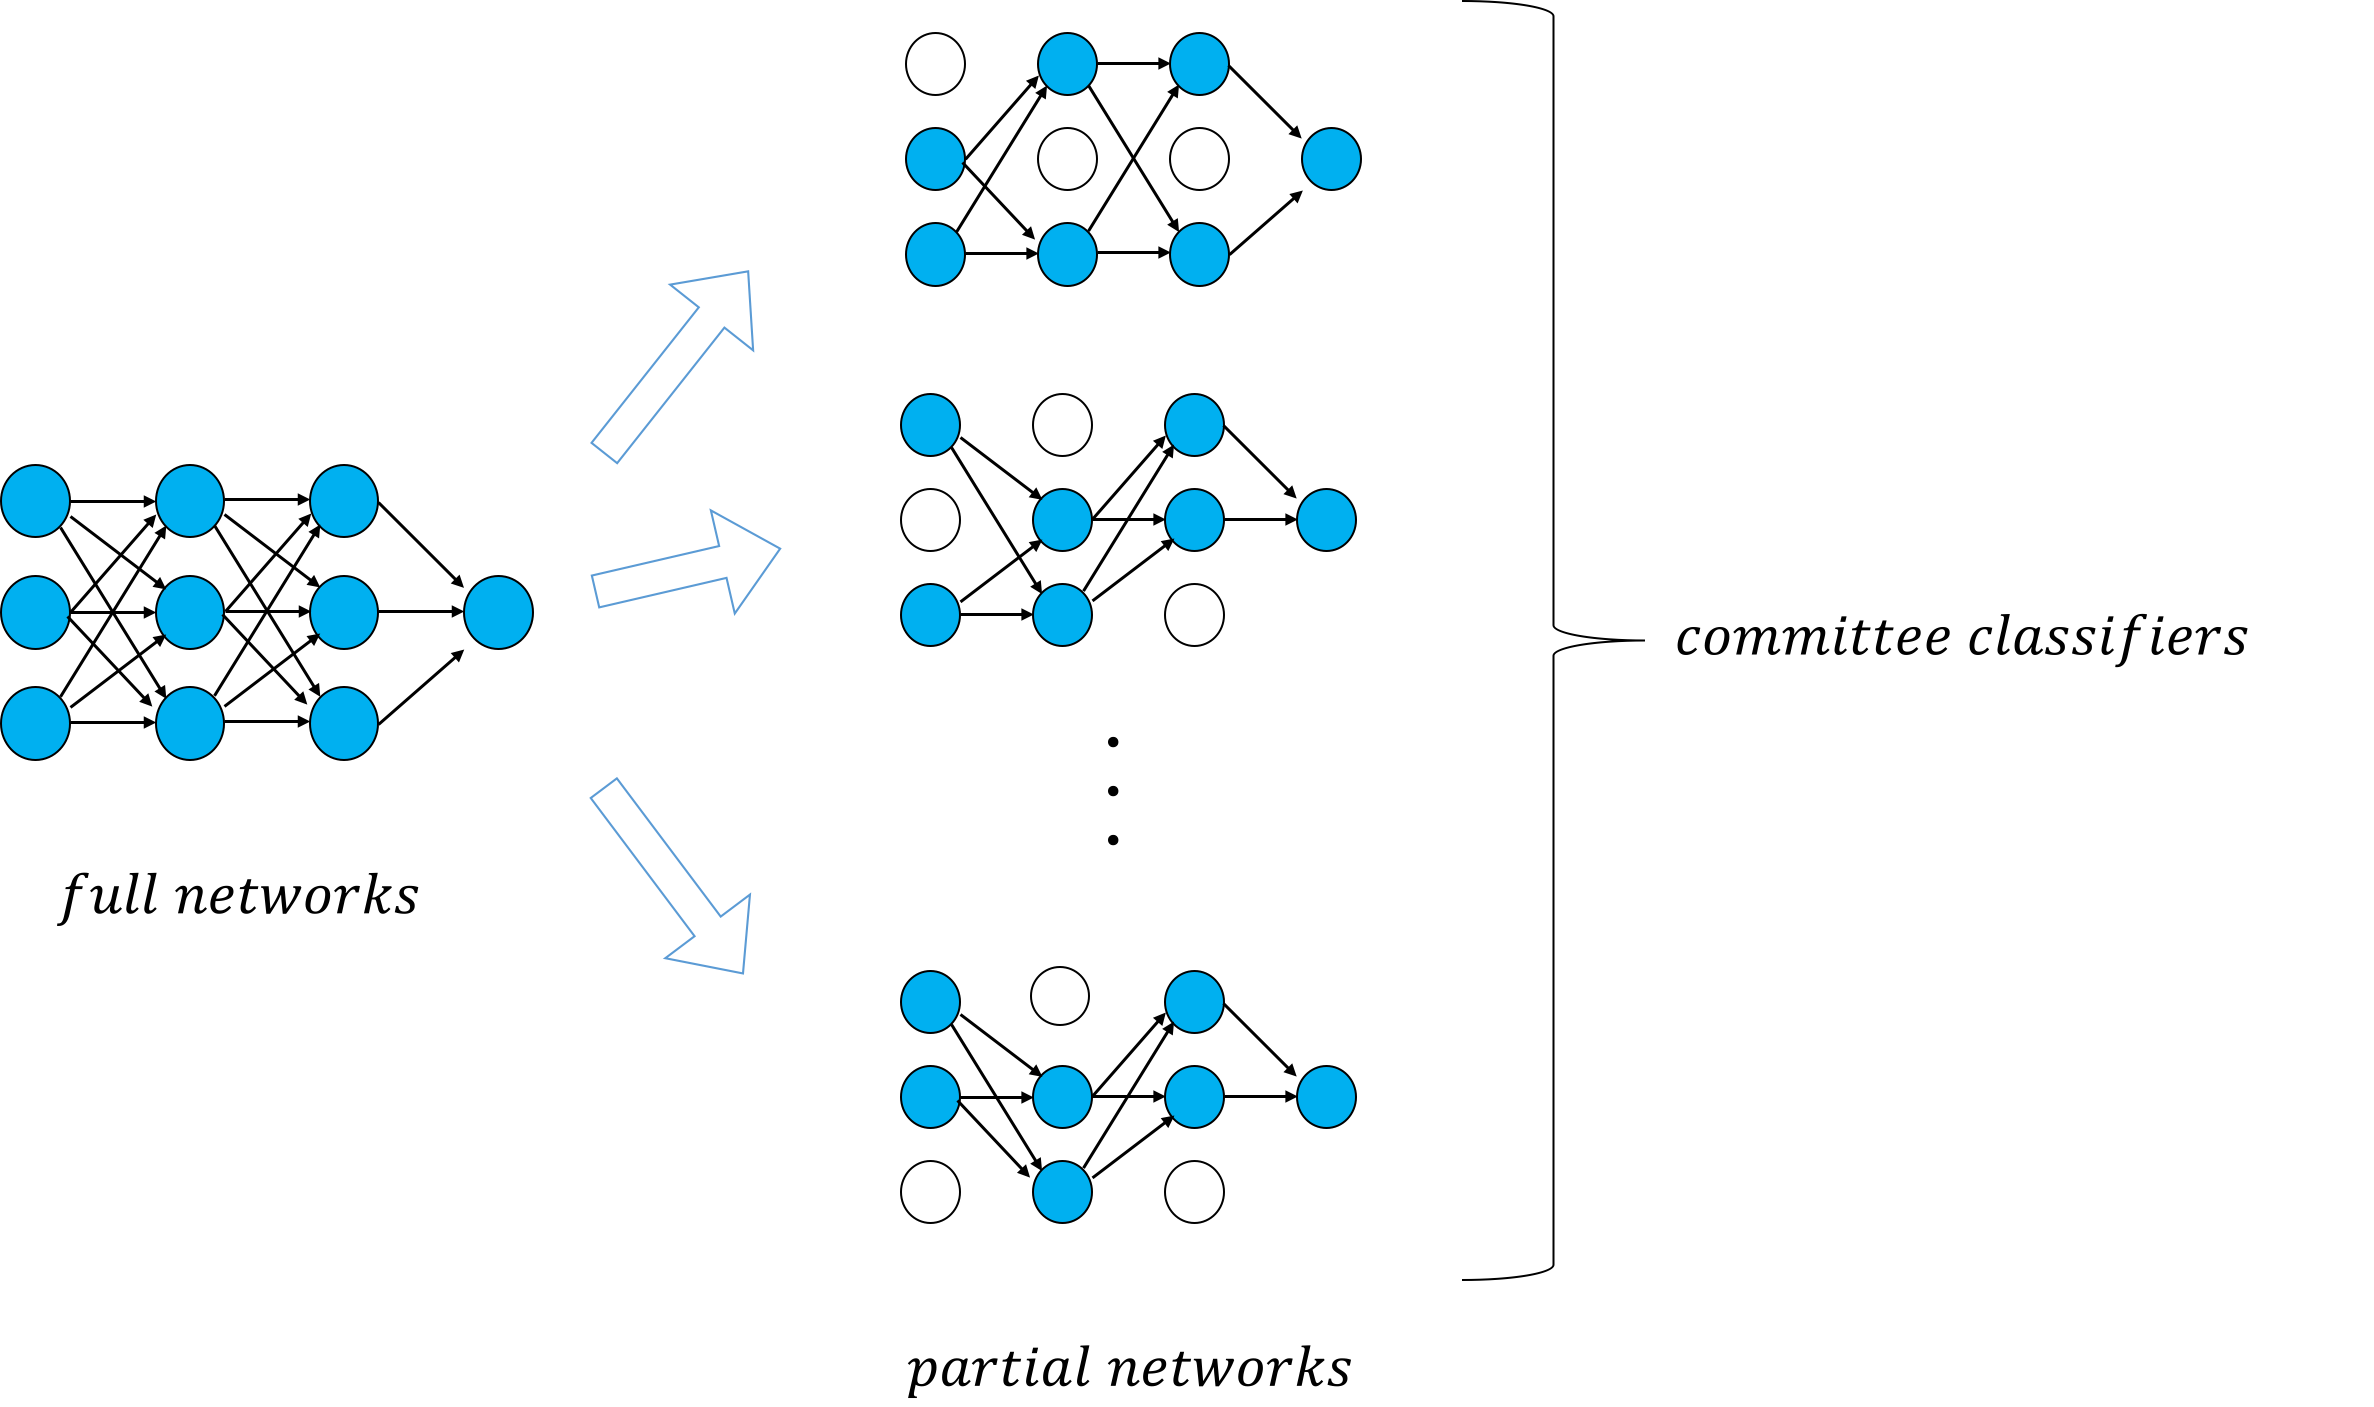
\includegraphics[width=120mm]{figures/query_by_dropout.png}
     \end{center}
    \caption{\label{fig:query_by_dropout}提案するQuery-By-Dropout-Predictionsの概要図.Dropoutによってサンプリングされた部分ネットワークによってCommitteeを形成する.}
\end{figure}

\subsection{推論時での\textbf{Data Augmentation}の利用}
CNNを学習させる際,訓練時に画像に対してData Augmentationを利用することで不変性を獲得させ,結果的に汎化性能を向上させる工夫が用いられる.
ラベル付きデータが少ない場合は特に過学習を防ぐために有効であると知られており,本研究でも識別器の学習に使用する.
第2章で述べたように,医療画像解析では一般画像認識と比較してモデルが獲得すべき不変性が多く存在する.
特に病理画像解析では,回転,位置に対する不変性,色相,輝度に対する不変性を獲得しているのが望ましい.

前項で,Dropoutによって生成された部分ネットワークによるCommitteeの不一致度を測る手法を提案したが,
本研究ではそれだけではなく,Data Augmentationを推論時にも利用することで,さらに効率的にモデルを更新するサンプルを選択する手法を提案する.
提案手法の動作原理のイメージ図を図\ref{fig:how_it_works}に示す.
通常Dropoutはネットワークの後段の全結合層のみで使用されることが多い.
すなわち,DropoutによってサンプリングされたCommitteeの各メンバは,CNNの畳み込み層から抽出された同一の特徴量に対する識別境界面の引き方が異なるのだと考えられる.
この時,Committeeの各メンバの予測の不一致度が高くなるようなサンプルは,Uncertain Samplingと比較して識別境界を大きく変更させるために有効であると考えられる.
しかしCNNにおいては,識別境界の決定だけでなく特徴抽出の表現学習も重要な因子である.
訓練時のみではなく不一致度の計算の際の推論時にもData Augmentationを利用すると,同一のサンプルが特徴空間上の異なる点に配置されると考えられる.
理想的にはそれらの点はすべて識別境界から見て同じ側に配置されるべきである.
そこで,推論時のDaga Augmentationを利用して予測が不一致したサンプルは,識別境界面を跨いでしまっているということであるので,
そのサンプルを学習することで,特徴抽出が頑健になるのではないかと考えられる.

結局,推論時にData AugmentationとDropoutを利用することで,識別境界の決定,特徴抽出の学習それぞれに有用であるサンプルが選択できるのではないかと考えられる.
これを実験で検証する.

\begin{figure}[tbp]
     \begin{center}
      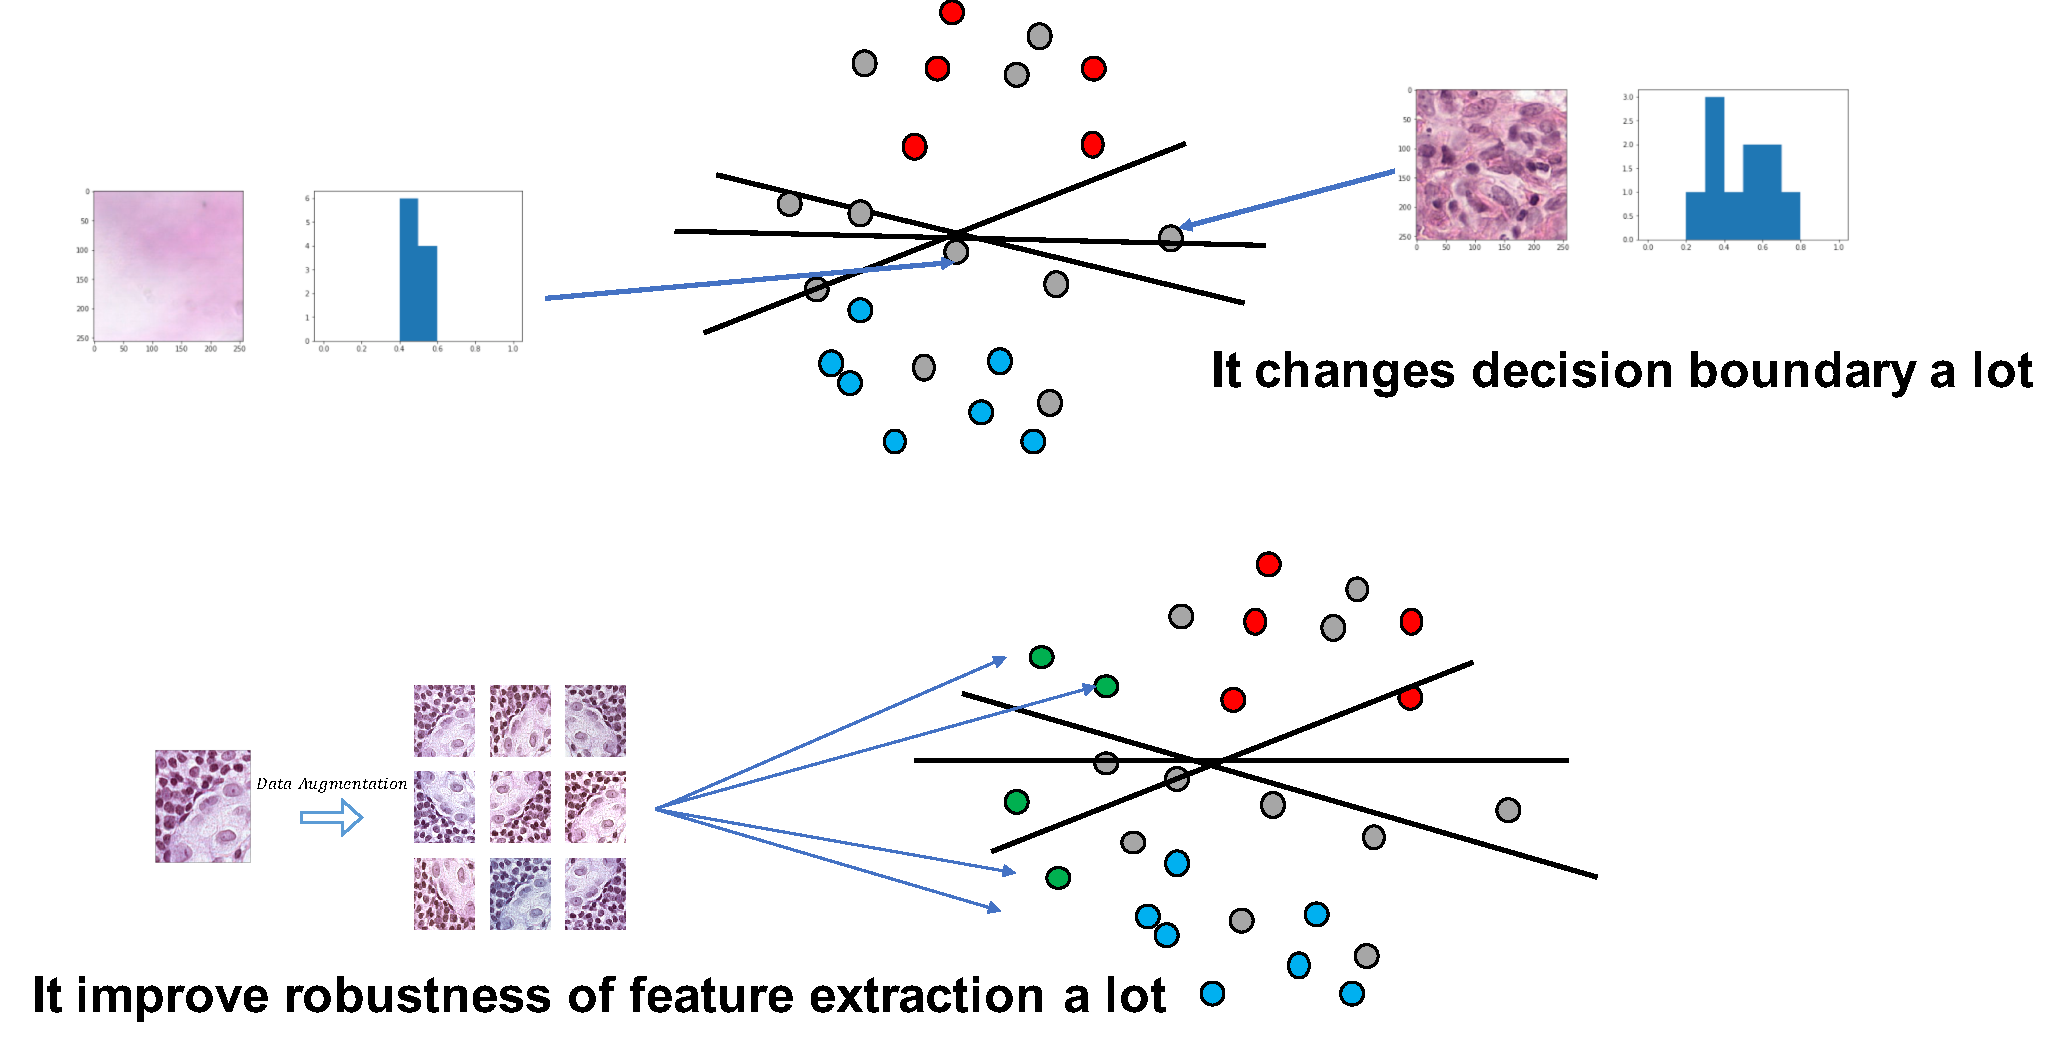
\includegraphics[width=120mm]{figures/how_it_works.pdf}
     \end{center}
    \caption{\label{fig:how_it_works}提案手法の動作原理のイメージ図.Dropoutによる不一致度の定量評価をData Augmentationを併用することで効果を高める.}
\end{figure}


\begin{algorithm}[h]
    \caption{Query-By-Dropout-Predicitions}
    \label{algo:qbdp}
    \begin{algorithmic}
        \STATE \textbf{Input: } 
        full network $\mathcal{M}$,
        unlabeled labeled datset $\mathcal{U}$,
        active sampling size $K$,
    \end{algorithmic}

    \begin{algorithmic}
        \STATE \textbf{Output: } query $\mathcal{Q}$
    \end{algorithmic}
    
    \begin{algorithmic}[1]
        \STATE sample Committee $\mathcal{C} = \{\mathcal{M}_{p_1}, \mathcal{M}_{p_2}, \dots, \mathcal{M}_{p_c} \}$ from $\mathcal{M}$ using $dropout$ 
        \FOR {$each \; x \in \mathcal{U}$}
            \STATE $score (x) \; = disagreement\_score \; (x, \; \mathcal{C}) $
        \ENDFOR
        \STATE $\mathcal{Q} \leftarrow \O$, $\mathcal{D} \leftarrow \O$
        \WHILE{$len(\mathcal{Q}) < K$}
        \STATE $x^{\ast} = \argmax_{x \in \mathcal{U}_i} score(x)$
        \STATE $idx = cluster(x^{\ast})$
        \IF{$idx \notin D$}
        \STATE $\mathcal{Q} \leftarrow \mathcal{Q} \cup \{x^{\ast}\}, \mathcal{D} \leftarrow \mathcal{D} \cup \{idx\}$
        \ENDIF
        \ENDWHILE
        \RETURN $\mathcal{Q}$
    \end{algorithmic}
  \end{algorithm}


\section{病理画像解析に適用するための工夫}
\subsection{ラベルなしデータプールのサンプリング}
病理画像解析ではWSIを複数の画像パッチに分割して扱うが,一般画像認識で用いられるようなサイズ($256 \times 256$)だと仮定すると,
1枚あたり数万〜数十万枚の画像パッチを含むことになる.
また,訓練時に使用できるWSIから全ての画像パッチを取り出しラベルなしデータセット$\mathcal{U}$として利用すろと,その数は数百万オーダーとなる.
このサンプルプールからあるクエリ選考基準を最大化するサンプルを選択するのは計算コストの点から実用上困難である.
しかし予め一定数をサンプリングして固定の$\mathcal{U}$を使用するのは,利用可能なデータ数を制限することになってしまう.
そこで,クエリ問い合わせ毎に利用可能な画像パッチ全体から一部をサンプリングすることで$\mathcal{U}_i$を作成し,
この中からモデル更新に寄与するサンプルを選択することで,現実時間内で最適なクエリを探索可能にしつつ,
利用可能データを最大限に利用する方法を提案する.
画像パッチをサンプリングする際は,各WSIから均等に選択する.
また,画像パッチの近傍は似た画像が多いことを考慮し,ある領域から2枚以上の画像パッチが選択されないように気をつけて行う.
さらに,一度選択された領域は次のサンプリングでは避けるようにする.

\subsection{バッチ型能動学習への拡張}
\ref{seq:al} 節で述べたように,能動学習ではクエリ問い合わせを行いラベルデータを拡充するごとに,識別器を初期値に戻してから再学習させるのが一般的である.
CNNを能動学習に利用する場合,一度の再学習に高い計算コストがかかってしまうため,
各クエリ問い合わせにおいて複数のサンプルにラベルを付与するバッチ型能動学習を採用するのが適当であると考えられる.
一度に投げるクエリ内での情報の重複を避けるために何らかの工夫をする必要があるが,
2章で述べたような劣モジュラ関数を設計するのは深層学習を利用する場合計算コストの観点から難しい.
そこで,本研究では予めラベルなしデータをクラスタリングし,一度のクエリでは同一のクラスターに属するサンプルを2つ以上選択しないことで,情報の重複を避ける.
ここでは,クラスタリング手法はアルゴリズムのシンプルさからk-meansに固定した.
クラスタリングに使用する特徴量の候補として,以下の3つを考慮した.

\subsubsection{\textbf{Hand-crafted feature}}
第2章で述べたように,病理画像解析にはテクスチャ解析で用いられる技術がしばしば使用される.
ここでは,パターンベースの特徴量で,位置不変性と輝度変化への頑健性を有するLocal Binary Pattern (LBP)\cite{ojala2002multiresolution}を採用する.
実際には,回転不変性を担保させるようにLBPを改良したimproved LBPを利用した.

\subsubsection{\textbf{CNN}の中間特徴量}
Imagenetで学習された特徴量は様々なタスクに有用であるとされており,多数の医療画像解析で利用されている.
本研究ではGoogleNet\cite{szegedy2015going}の中間特徴量を空間方向に平均を取ることで圧縮した512次元を利用した.

\subsubsection{\textbf{Compact Bilinear Pooling}による特徴量}
近年では,深層学習を用いたテクスチャ解析に関する研究も盛んに行われている.
Bilinear Pooling \cite{lin2015bilinear}は,CNNの中間特徴量同士の相関を計算し空間方向に平均を取ることで獲得される自己相関行列を特徴量として利用する手法である.
\begin{eqnarray}
G_{ij} = \sum_k{F_{ik} F_{jk}}
\end{eqnarray}
$G$はBilinear Poolingによって得られる自己相関行列,$F$はCNNの中間特徴マップ,$k$は画像中の位置情報を表す.
一般にCNNの特徴量次元(チャンネル数)は256 〜 512の大きな値であるため,直接計算した場合非常に高次元な値となってしまう.
そこで,ランダム行列によってBilinear Poolingによって得られる特徴量を近似する手法である
Compact Bilinear Pooling(CBP)\cite{gao2016compact}を本研究では採用する.
ランダム行列の次元を増やすほどBilinear Poolingの近似精度が上がるという特徴になっている.
CNNを用いたテクスチャ特徴量として,GoogleNet\cite{szegedy2015going}の中間特徴量をCBPによって512次元まで圧縮したものを採用する.

\section{アルゴリズムの詳細}

本研究で提案するアルゴリズムの詳細を以下に示す(Algorithm\ref{algo:dal}).

\begin{description}
    \item[step1] ラベルなしデータセット$\mathcal{U}$,初期ラベル付きデータセット$\mathcal{L}$を準備する
    \item[step2] CNNモデル$\mathcal{M}$に学習済みモデルの重みをセットする
    \item[step3] $\mathcal{L}$を利用して,$\mathcal{M}$をfine-tuningにより学習
    \item[step4] $\mathcal{U}$から$\mathcal{U}_i$をサンプリングする
    \item[step5] K-meansによって$\mathcal{U}_i$を$\mathcal{U}_{i_1}, \mathcal{U}_{i_2}, \dots, \mathcal{U}_{i_k}$にクラスタリングする
    \item[step6] Dropoutにより$\mathcal{L}$からCommittee $\mathcal{C} = \{\mathcal{M}_{p_1}, \mathcal{M}_{p_2}, \dots, \mathcal{M}_{p_c} \}$を生成
    \item[step7] Committee $\mathcal{C}$ を利用し$\mathcal{U}$のdisagreement scoreを計算
    \item[step8] $\mathcal{U}$からスコアが高いものを,同一クラスターからは2つ以上選択しないように選び,クエリ$Q$を作成
    \item[step9] $Q$にラベルを付与し,$\mathcal{L}$に追加する
    \item[step10] モデルのvalidation scoreが望みの値を達成するまでstep3〜step9を繰り返す
\end{description}


\begin{algorithm}[h]
    \caption{Deep Active Learning for Pathological Image Analysis}
    \label{algo:dal}
    \begin{algorithmic}
        \STATE \textbf{Input: } 
        unlabeled dataset $\mathcal{U}$,
        initial labeled datset $\mathcal{L}$,
        clustering size $k$, 
        active sampling size $K$,
    \end{algorithmic}

    \begin{algorithmic}
        \STATE \textbf{Output: } paramters of network $\mathcal{M}$
    \end{algorithmic}

    \begin{algorithmic}[1]
        \STATE Initialize pre-trained network $\mathcal{M}_{pretrained}$
        \REPEAT
            \STATE $\mathcal{M} \leftarrow train (\mathcal{M}_{pretrained}, \mathcal{L})$
            \STATE sample partial unlabeled dataset $\mathcal{U}_i$ from $\mathcal{U}$
            \STATE Perform k-means clustering and devide $\mathcal{U}_i$ to disjoint clusters $\mathcal{U}_{i_1}, \mathcal{U}_{i_2}, \dots, \mathcal{U}_{i_k}$
            \STATE $\mathcal{Q} \leftarrow QBDP(\mathcal{M}, \mathcal{U}_i, K)$
            \STATE Query labels for $\mathcal{Q}$
            \STATE $\mathcal{L} \leftarrow \mathcal{L} \cup \mathcal{Q}$

      \UNTIL{perfomance is satisfactory}
    \end{algorithmic}
  \end{algorithm}
  
